\documentclass[
	12pt,				% tamanho da fonte
	oneside,			% p/ impressão frente e verso:
	a4paper,			% tamanho do papel. 
	english,			% idioma adicional para hifenização
	french,				% idioma adicional para hifenização
	spanish,			% idioma adicional para hifenização
	brazil				% o último idioma é o principal do documento
	]{abntex2}
% ---
% Pacotes básicos 
% ---
\usepackage{lmodern}			% Usa a fonte Latin Modern			
\usepackage[T1]{fontenc}		% Selecao de codigos de fonte.
\usepackage[utf8]{inputenc}		% Codificacao do documento (conversão automática dos acentos)
\usepackage{indentfirst}		% Indenta o primeiro parágrafo de cada seção.
\usepackage{color}				% Controle das cores
\usepackage{graphicx}			% Inclusão de gráficos
\usepackage{microtype} 			% para melhorias de justificação
\usepackage{xspace}             % Para símbolo como \latex

% ---
% Pacotes Matlab 
% ---
\usepackage[framed, numbered]{matlab-prettifier}
\newcommand{\MATLAB}{MATLAB\textsuperscript{\textregistered}\xspace}

% Pacotes necessários:
%\usepackage{xcolor} % Controle de Cores
%\usepackage{listings} %Para inserir o código

\definecolor{verde}{rgb}{0,0.5,0} % Definindo novas cores

% Configurando layout para mostrar códigos C
\lstset{
  language=C,
  basicstyle=\ttfamily\small, 
  keywordstyle=\color{blue}, 
  stringstyle=\color{verde}, 
  commentstyle=\color{red}, 
  extendedchars=true, 
  showspaces=false, 
  showstringspaces=false, 
  numbers=left,
  numberstyle=\tiny,
  breaklines=true, 
  backgroundcolor=\color{green!10},
  breakautoindent=true, 
  captionpos=b,
  xleftmargin=0pt,
}

\lstset{literate=%
            {á}{{\'a}}{1}%
            {à}{{\`a}}{1}%
            {ã}{{\~a}}{1}%
            {â}{{\^a}}{1}%
            {é}{{\'e}}{1}%
            {è}{{\`e}}{1}%
            {ê}{{\^e}}{1}%
            {í}{{\'i}}{1}%
            {ó}{{\'o}}{1}%
            {ô}{{\^o}}{1}%
            {ò}{{\`o}}{1}%
            {õ}{{\~o}}{1}%
            {ú}{{\'u}}{1}%
            {ç}{{\c{c}}}{1}%
            {Á}{{\'A}}{1}%
            {À}{{\`A}}{1}%
            {Â}{{\^A}}{1}%
            {Ã}{{\~A}}{1}%
            {É}{{\'E}}{1}%
            {È}{{\`E}}{1}%
            {Ê}{{\^E}}{1}%
            {Í}{{\'I}}{1}%
            {Ó}{{\'O}}{1}%
            {Ô}{{\^O}}{1}%
            {Ò}{{\`O}}{1}%
            {Õ}{{\~O}}{1}%
            {Ú}{{\'U}}{1}%
            {Ç}{{\c C}}{1}%
}

% ---
% Atribuições Matemáticas 
% ---
\usepackage{amsmath, amsfonts, amssymb} % pacotes para caracteres extras
\DeclareMathOperator{\sen}{sen}
\DeclareMathOperator{\arcsen}{arcsen}
\DeclareMathOperator{\tg}{tg}
\DeclareMathOperator{\cossec}{cossec}
\newcommand{\limite}{\displaystyle\lim}
\newcommand{\integral}{\displaystyle\int}
		
% ---
% Pacotes de citações
% ---
\usepackage[brazilian,hyperpageref]{backref}	 % Paginas com as citações na bibl
\usepackage[alf]{abntex2cite}	% Citações padrão ABNT

% --- 
% CONFIGURAÇÕES DE PACOTES
% --- 
% Configurações do pacote backref
% Usado sem a opção hyperpageref de backref
\renewcommand{\backrefpagesname}{Citado na(s) página(s):~}
% Texto padrão antes do número das páginas
\renewcommand{\backref}{}
% Define os textos da citação
\renewcommand*{\backrefalt}[4]{
	\ifcase #1 %
		Nenhuma citação no texto.%
	\or
		Citado na página #2.%
	\else
		Citado #1 vezes nas páginas #2.%
	\fi}%
% ---

% ---
% Informações de dados para CAPA e FOLHA DE ROSTO
% ---
\titulo{Projeto Computacional: \\ \textbf{Solução de Sistemas Não-Lineares via Métodos de Newton-Raphson e Quasi-Newton Usando o \textbf{\MATLAB}}}
\autor{Antonio Gabriel Sousa Borralho\\Arthur Monteiro Costa Silva\\Cesar Eugenio Cunha de Carvalho\\Evelyn Cristina de Oliveira Lima\\Gilberto Balby Araujo Filho\\Lucas Costa Soares\\}
\local{São Luís, MA - Brasil}
\data{\today}
%\orientador{Prof. Professor}
\tipotrabalho{Trabalho Acadêmico}
% O preambulo deve conter o tipo do trabalho, o objetivo, 
% o nome da instituição e a área de concentração 
\preambulo{Trabalho referente ao desenvolvimento de um projeto computacional para obtenção da terceira nota da disciplina Métodos Numéricos e Otimização no período de 2018.1.\newline \newline Prof. Anselmo Barbosa Rodrigues.}
% ---


% Configurações de aparência do PDF final

% alterando o aspecto da cor azul
\definecolor{blue}{RGB}{41,5,195}

% informações do PDF
\makeatletter

\hypersetup{
     	%pagebackref=true,
		pdftitle={\@title}, 
		pdfauthor={\@author},
    	%pdfsubject={\imprimirpreambulo},
	    pdfcreator={LaTeX with abnTeX2},
		pdfkeywords={abnt}{latex}{abntex}{abntex2}{trabalho acadêmico}, 
		colorlinks=true,       		% false: boxed links; true: colored links
    	linkcolor=blue,          	% color of internal links
    	citecolor=blue,        		% color of links to bibliography
    	filecolor=magenta,          % color of file links
		urlcolor=blue,
		bookmarksdepth=4
}

\makeatother
% --- 

% --- 
% Espaçamentos entre linhas e parágrafos 
% --- 

% O tamanho do parágrafo é dado por:
\setlength{\parindent}{1.3cm}

% Controle do espaçamento entre um parágrafo e outro:
\setlength{\parskip}{0.2cm}  % tente também \onelineskip

% ---
% compila o indice
% ---
\makeindex
% ---

% ----
% Início do documento
% ----
\begin{document}

% Seleciona o idioma do documento (conforme pacotes do babel)
%\selectlanguage{english}
\selectlanguage{brazil}

% Retira espaço extra obsoleto entre as frases.
\frenchspacing 

% ----------------------------------------------------------
% ELEMENTOS PRÉ-TEXTUAIS
% ----------------------------------------------------------
\pretextual
% ---
% --------------------- CAPA -------------------------------
% ---
\begin{center}			
	\begin{figure}[htb]
		\centering
		
\includegraphics[scale=0.15]{ufmalogo.jpg}
	\end{figure}
				
			\textbf{UNIVERSIDADE FEDERAL DO MARANHÃO \\
					CENTRO DE CIÊNCIAS EXATAS E TECNOLOGIAS \\
					DEPARTAMENTO DE ENGENHARIA ELÉTRICA \\
				    MÉTODOS NUMÉRICOS E OTIMIZAÇÃO\\\vspace{4cm}}
					
					\textbf{\large{Projeto Computacional:}}\\
					\large{Solução de Sistemas Não-Lineares via Métodos de Newton-Raphson e Quasi-Newton Usando o \textbf{\MATLAB}}
					\vspace{2.5cm}
					\begin{flushright}
						\textnormal{Antonio Gabriel Sousa Borralho\\Arthur Monteiro Costa Silva\\Cesar Eugenio Cunha de Carvalho\\Evelyn Cristina de Oliveira Lima\\Gilberto Balby Araujo Filho\\Lucas Costa Soares\\}
					\end{flushright}
					\vspace{2.5cm}
					\textbf{São Luís, MA - Brasil\\ \today}
\end{center}
% ---
% --------------------- FOLHA DE ROSTO -------------------------------
% ---
\renewcommand{\folhaderostocontent}{  % Cria sua própria folha de rosto 
    \begin{center}
        % ____Autores_________________________________________
        {\ABNTEXchapterfont\imprimirautor}
        \vspace*{\fill}\vspace*{\fill}
        % ____Título_________________________________________
        \begin{center}
            \ABNTEXchapterfont\bfseries\Large\imprimirtitulo
        \end{center}
        \vspace*{\fill}
        % ____Pré-Ambulo_________________________________________
        \abntex{}{%
            \hspace{.45\textwidth}
            \begin{minipage}{.5\textwidth}
                \SingleSpacing
                \imprimirpreambulo
            \end{minipage}%
            \vspace*{\fill}
        }%
        {\large\imprimirlocal}
        \par
        {\large\imprimirdata}
        %\vspace*{1cm}
    \end{center}
}
\makeatother
% ---
% Folha de rosto
% ---
\imprimirfolhaderosto

% ---
% --------------------- SUMÁRIO -------------------------------
% ---
\pdfbookmark[0]{\contentsname}{toc}
\tableofcontents*
\cleardoublepage
% ---

% ----------------------------------------------------------
% ELEMENTOS TEXTUAIS
% ----------------------------------------------------------
\textual
% ----------------------------------------------------------
% Introdução
% ----------------------------------------------------------
\chapter{Introdução}\index{introdução}
% ----------------------------------------------------------
Muitos problemas da engenharia, física e matemática estão associados à solução de sistemas de equações lineares. Nesse contexto, tratamos de técnicas numéricas empregadas para obter a solução desses sistemas. Iniciamos por uma rápida revisão do método de eliminação gaussiana do ponto de vista computacional. No contexto de análise da propagação dos erros de arredondamento, introduzimos o método de eliminação gaussiana com pivotamento parcial, bem como, apresentamos o conceito de condicionamento de um sistema linear. Além disso, exploramos o conceito de complexidade de algoritmos em álgebra linear. Então, passamos a discutir sobre técnicas iterativas, mais especificamente, sobre os métodos de \textbf{Newton-Raphson} e \textbf{Quasi-Newton} para a solução de sistemas de equações não-lineares.\cite{neide}.
%\textbf{\MATLAB}\footnote{\url{<https://www.mathworks.com MathWorks> }} 

\section{Solução de sistemas lineares}\index{sistema linear}

Considere o sistema de equações lineares (escrito na forma algébrica)
\begin{equation}
  \begin{split}
    a_{11}x_1 + a_{12}x_2 + \cdots +a_{1n}x_n &= b_1\\
    a_{21}x_1 + a_{22}x_2 + \cdots +a_{2n}x_n &= b_2\\
    &\vdots \\
    a_{m1}x_1 + a_{m2}x_2 + \cdots +a_{mn}x_n &= b_m
  \end{split}
\end{equation}
onde $m$ é o número de equações e $n$ é o número de incógnitas.  Este sistema pode ser escrito na \emph{forma matricial}
\begin{equation}
  Ax = b
\end{equation}
onde:
\begin{equation}
  A=\begin{bmatrix}
a_{11} & a_{12} & \cdots & a_{1n}\\
a_{21} & a_{22} & \cdots & a_{2n}\\
\vdots & \vdots & \ddots & \vdots\\
a_{m1} & a_{m2} & \cdots & a_{mn}
\end{bmatrix},
x=\begin{bmatrix}
x_{1} \\
x_{2} \\
\vdots \\
x_{n}
\end{bmatrix}
 \text{ e } b=\begin{bmatrix}
b_{1} \\
b_{2} \\
\vdots \\
b_{m}
\end{bmatrix},
\end{equation}
onde $A$ é chamada de \emph{matriz dos coeficientes}\index{matriz!dos coeficientes}, $x$ de \emph{vetor das incógnitas}\index{vetor!das incógnitas} e $b$ de \emph{vetor dos termos constantes}\index{vetor!dos termos constantes}.


Definimos também a \emph{matriz completa}\index{matriz!completa} (também chamada de \emph{matriz estendida}\index{matriz!estendida}) de um sistema como $Ax=b$ como $[A|b]$, isto é
\begin{equation}
 [A|b]=\left[\begin{array}{cccc|c}
a_{11} & a_{12} & \cdots & a_{1n}&b_1\\
a_{21} & a_{22} & \cdots & a_{2n}&b_2\\
\vdots & \vdots & \ddots & \vdots&\vdots\\
a_{m1} & a_{m2} & \cdots & a_{mn}&b_m
\end{array}\right]
\end{equation}


Salvo especificado ao contrário, assumiremos ao longo deste capítulo que a matriz dos coeficientes $A$ é uma matriz real não singular (isto é, invertível).

\section{Eliminação de Gauss}\index{eliminação gaussiana}
A \emph{eliminação gaussiana}, também conhecida como \emph{escalonamento}, é um método para resolver sistemas lineares. Este método consiste em manipular o sistema através de determinadas operações elementares, transformando a matriz estendida do sistema em uma matriz triangular (chamada de \emph{matriz escalonada do sistema}\index{matriz escalonada})\cite{ufpb}. Uma vez, triangularizado o sistema, a solução pode ser obtida via substituição regressiva \cite{neide}. Naturalmente estas operações elementares devem preservar a solução do sistema e consistem em:
\begin{enumerate}
\item multiplicação de um linha por uma constante não nula.
\item substituição de uma linha por ela mesma somada a um múltiplo de outra linha.
\item permutação de duas linhas.
\end{enumerate}

\begin{ex}\label{ex:elim_gaussiana} Resolva o sistema
  \begin{equation}
    \begin{split}
      x+y+z  &= 1\\
      4x+4y+2z&= 2\\
      2x+y-z &= 0
    \end{split}
  \end{equation}
pelo método de eliminação gaussiana.
\end{ex}
\begin{sol}
A matriz estendida do sistema é escrita como
\begin{equation}
  \begin{bmatrix}
      1 &1& 1&1\\
      4 & 4 &2&2\\
      2 &1& -1&0
  \end{bmatrix}
\end{equation}
No primeiro passo, subtraímos da segunda linha o quádruplo da primeira e subtraímos da terceira linha o dobro da primeira linha:
\begin{equation}
  \begin{bmatrix}
       1 &1& 1&1\\
       0 & 0 &-2&-2\\
       0 &-1& -3&-2
  \end{bmatrix}
\end{equation}
No segundo passo, permutamos a segunda linha com a terceira:
\begin{equation}
  \begin{bmatrix}
       1 &1& 1&1\\
       0 &-1& -3&-2\\
       0 & 0 &-2&-2
  \end{bmatrix}
\end{equation}
Neste momento, a matriz já se encontra na forma triangular (chamada de \emph{matriz escalonada do sistema}\index{matriz escalonada}). Da terceira linha, encontramos $-2z=-2$, ou seja, $z=1$. Substituindo na segunda equação, temos $-y-3z=-2$, ou seja, $y=-1$ e finalmente, da primeira linha, $x+y+z=1$, resultando em $x=1$.
\end{sol}

Neste Exemplo~\ref{ex:elim_gaussiana}, o procedimento de eliminação gaussiana foi usado para obtermos um sistema triangular (superior) equivalente ao sistema original. Este, por sua vez, nos permitiu calcular a solução do sistema, isolando cada variável, começando da última linha (última equação), seguindo linha por linha até a primeira.

Alternativamente, podemos continuar o procedimento de eliminação gaussiana, anulando os elementos da matriz estendida acima da diagonal principal. Isto nos leva a uma matriz estendida diagonal (chamada \emph{matriz escalonada reduzida}\index{matriz escalonada reduzida}), na qual a solução do sistema original aparece na última coluna.

\begin{ex}
  No Exemplo~\ref{ex:elim_gaussiana}, usamos o procedimento de eliminação gaussiana e obtivemos
  \begin{equation}
      \underbrace{
        \begin{bmatrix}
          1 & 1 & 1 & 1\\
          4 & 4 & 2 & 2\\
          2 & 1 & -1 & 0
        \end{bmatrix}
}_{\text{matriz estendida}} \sim
      \underbrace{
        \begin{bmatrix}
          1 & 1 & 1 & 1\\
          0 & -1 & -3 & -2\\
          0 & 0 & -2 & -2
        \end{bmatrix}
}_{\text{matriz escalonada}}.
  \end{equation}

Agora, seguindo com o procedimento de eliminação gaussiana, buscaremos anular os elementos acima da diagonal principal. Começamos dividindo cada elemento da última linha pelo valor do elemento da sua diagonal, obtemos
\begin{equation}
  \begin{bmatrix}
    1 & 1 & 1 & 1\\
    0 & -1 & -3 & -2\\
    0 & 0 & 1 & 1
  \end{bmatrix}
\end{equation}
Então, somando da segunda linha o triplo da terceira e subtraindo da primeira a terceira linha, obtemos
\begin{equation}
  \begin{bmatrix}
    1 & 1 & 0 & 0\\
    0 & -1 & 0 & 1\\
    0 & 0 & 1 & 1
  \end{bmatrix}
\end{equation}
Fixamos, agora, na segunda linha. Dividimos esta linha pelo valor do elemento em sua diagonal, isto nos fornece
\begin{equation}
  \begin{bmatrix}
    1 & 1 & 0 & 0\\
    0 & 1 & 0 & -1\\
    0 & 0 & 1 & 1
  \end{bmatrix}
\end{equation}
Por fim, subtraímos da primeira linha a segunda, obtendo a matriz escalonada reduzida
\begin{equation}
  \begin{bmatrix}
    1 & 0 & 0 & 1\\
    0 & 1 & 0 & -1\\
    0 & 0 & 1 & 1
  \end{bmatrix}
\end{equation}
Desta matriz escalonada reduzida temos, imediatamente, $x=1$, $y=-1$ e $z=1$, como no Exemplo~\ref{ex:elim_gaussiana}.
\end{ex}

\subsection{Eliminação gaussiana com pivotamento parcial}
A eliminação gaussiana com \emph{pivotamento parcial} consiste em fazer uma permutação de linhas de forma a escolher o maior pivô (em módulo) a cada passo \cite{neide}.

\begin{ex} Resolva o sistema
\begin{equation}
  \begin{split}
    x+y+z  &= 1\\
    2x+y-z &= 0\\
    2x+2y+z &= 1
  \end{split}
\end{equation}
por eliminação gaussiana com pivotamento parcial.
\end{ex}
\begin{sol}
A matriz estendida do sistema é
\begin{equation}
  \begin{split}
    \begin{bmatrix}
      1 &1&  1&1\\
      \BLU{2} &1& -1&0\\
      2 & 2 &1&1
    \end{bmatrix}
    &\sim
    \begin{bmatrix}
      \BLU{2} &1& -1&0\\
      1 &1&  1&1\\
      2 &2&  1&1
    \end{bmatrix}\\
    &\sim
    \begin{bmatrix}
      2 &1& -1&0\\
      0 &1/2& 3/2&1\\
      0 & 1 &2&1
    \end{bmatrix}\\
    &\sim
    \begin{bmatrix}
      2 &1& -1&0\\
      0 & 1 &2&1\\
      0 &1/2& 3/2&1
    \end{bmatrix}\\
    &\sim
    \begin{bmatrix}
      2 &1& -1&0\\
      0 & 1 &2&1\\
      0 &0& 1/2&1/2
    \end{bmatrix}
  \end{split}
\end{equation}
Encontramos $1/2z=1/2$, ou seja, $z=1$. Substituímos na segunda equação e temos $y+2z=1$, ou seja, $y=-1$ e, finalmente $2x+y-z=0$, resultando em $x=1$.
\end{sol}

A técnica de eliminação gaussiana com pivotamento parcial ajuda a evitar a propagação dos erros de arredondamento.

\section{Sistemas triangulares}
Considere um sistema linear onde a matriz é triangular superior, ou seja,
\begin{equation}\begin{bmatrix}
a_{11} & a_{12} & \cdots & a_{1n}\\
0      & a_{22} & \cdots & a_{2n}\\
\vdots & \vdots & \ddots & \vdots\\
0      & \dots  & 0     & a_{nn}
\end{bmatrix}
\begin{bmatrix}
x_{1} \\
x_{2} \\
\vdots \\
x_{n}
\end{bmatrix}
 =\begin{bmatrix}
b_{1} \\
b_{2} \\
\vdots \\
b_{n}
\end{bmatrix}
\end{equation}
tal que todos elementos abaixo da diagonal são iguais a zero.

Podemos resolver esse sistema iniciando pela última equação e isolando $x_n$ obtemos
\begin{equation}
 x_n = b_n/a_{nn}
\end{equation}

Substituindo $x_n$ na penúltima equação
\begin{equation}
 a_{n-1,n-1}x_{n-1}+a_{n-1,n}x_n = b_{n-1}
\end{equation}
e isolando $x_{n-1}$ obtemos
\begin{equation}
 x_{n-1} = (b_{n-1}-a_{n-1,n}x_n)/a_{n-1,n-1}
\end{equation}
e continuando desta forma até a primeira equação obteremos
\begin{equation}
 x_{1} = (b_{1}-a_{12}x_2 \cdots -a_{1n}x_n)/a_{11}.
\end{equation}
De forma geral, temos que
\begin{equation}
 x_{i} = (b_{i}-a_{i,i+1}x_{i+1} \cdots -a_{i,n}x_n)/a_{i,i}, \quad i=2,\dots,n.
\end{equation}

\section{Gauss-LU}
Considere um sistema linear $Ax = b$, onde a matriz $A$ é densa\footnote{Diferentemente de uma matriz esparsa, uma matriz densa possui a maioria dos elementos diferentes de zero.}. A fim de resolver o sistema, podemos fatorar a matriz $A$ como o produto de uma matriz $L$ triangular inferior e uma matriz $U$ triangular superior, ou seja, $A=LU$ \cite{neide}.

Sendo assim, o sistema pode ser reescrito da seguinte forma:
\begin{eqnarray}
  Ax &=&b \\
  (LU)x &=&b \\
  L(Ux) &=&b \\
  L y = b \quad & \text{ e }& \quad Ux=y
\end{eqnarray}
Isto significa que, ao invés de resolvermos o sistema original, podemos resolver o sistema triangular inferior $Ly=b$ e, então, o sistema triangular superior $Ux = y$, o qual nos fornece a solução de $Ax = b$.

A matriz $U$ da fatoração\footnote{Não vamos usar pivotamento nesse primeiro exemplo.} $LU$ é a matriz obtida ao final do escalonamento da matriz $A$.

A matriz $L$ é construída  a partir da matriz identidade $I$, ao longo do escalonamento de A. Os elementos da matriz $L$ são os múltiplos do primeiro elemento da linha de $A$ \underline{a ser zerado} dividido pelo pivô acima na mesma coluna.

Por exemplo, para zerar o primeiro elemento da segunda linha de $A$, calculamos
\begin{equation} L_{21} = A_{21}/A_{11} \end{equation}
e fazemos
\begin{equation} A_{2,:} \Leftarrow A_{2,:} - L_{21}A_{1,:} \end{equation}

Note que denotamos $A_{i,:}$ para nos referenciarmos a linha $i$ de $A$. Da mesma forma, se necessário usaremos $A_{:,j}$ para nos referenciarmos a coluna $j$ de $A$.

Para zerar o primeiro elemento da terceira linha de $A$, temos
\begin{equation} L_{31}=A_{31}/A_{11} \end{equation}
e fazemos
\begin{equation} A_{3,:} \Leftarrow A_{3,:} - L_{31}A_{1,:} \end{equation}
até chegarmos ao último elemento da primeira coluna de $A$.

Repetimos o processo para as próximas colunas, escalonando a matriz $A$ e coletando os elementos $L_{ij}$ abaixo da diagonal\footnote{Perceba que a partir da segunda coluna para calcular $L_{ij}$ não usamos os elementos de $A$, mas os elementos da matriz $A$ em processo de escalonamento}.

\begin{ex}
  Use a fatoração LU para resolver o seguinte sistema linear:
  \begin{equation}
    \begin{split}
      x_1 + x_2 + x_3 &= -2\\
      2x_1 + x_2 - x_3 &= 1\\
      2x_1 -x_2 + x_3 &= 3
    \end{split}
  \end{equation}
\end{ex}
\begin{sol}
Começamos fatorando a matriz $A$ dos coeficientes deste sistema:
\begin{eqnarray}
      A =
    \begin{bmatrix}
      1 & 1 & 1\\
      2 & 1 & -1\\
      2 & -1 & 1
    \end{bmatrix}.
    &=&
     \underbrace{\begin{bmatrix}
      1 & 0 & 0\\
      0 & 1 & 0\\
      0 & 0 & 1
    \end{bmatrix}}_{I_{3,3}}
    \underbrace{\begin{bmatrix}
      1 & 1 & 1\\
      2 & 1 & -1\\
      2 & -1 & 1
    \end{bmatrix}}_{A}\\
  &=&
    \begin{bmatrix}
      1 & 0 & 0\\
      2 & 1 & 0\\
      2 & 0 & 1
    \end{bmatrix}
    \begin{bmatrix}
      1 & 1 & 1\\
      0 & -1 & -3\\
      0 & -3 & -1
    \end{bmatrix}\\
  &=&
    \underbrace{\begin{bmatrix}
      1 & 0 & 0\\
      2 & 1 & 0\\
      2 & 3 & 1
    \end{bmatrix}}_{L}
    \underbrace{\begin{bmatrix}
      1 & 1 & 1\\
      0 & -1 & -3\\
      0 & 0 & 8
    \end{bmatrix}}_{U}\\
\end{eqnarray}

Completada a fatoração LU, resolvemos, primeiramente, o sistema $Ly = b$:
\begin{equation}
  \begin{split}
    y_1 &= -2\\
    2y_1 + y_2 &= 1\\
    2y_1 + 3y_2 + y_3 &= 3
  \end{split}
\end{equation}
o qual no fornece $y_1 = -2$, $y_2 = 5$ e $y_3 = -8$. Por fim, obtemos a solução resolvendo o sistema $Ux = y$:
\begin{equation}
  \begin{split}
  x_1 + x_2 + x_3 &= -2\\
  -x_2 - 3x_3 &= 5\\
  8x_3 &= -8
  \end{split}
\end{equation}
o qual fornece $x_3 = -1$, $x_2 = -2$ e $x_1 = 1$.
\end{sol}

\subsection{Custo computacional para solução de um sistema linear usando Gauss-LU}
Para calcularmos o custo computacional de um algoritmo completo, uma estratégia é separar o algoritmo em partes menores, mais fáceis de analisar.

Para resolver o sistema, devemos primeiro fatorar a matriz $A$ nas matrizes $L$ e $U$. Vimos que o custo é
\begin{equation} \dfrac{2n^3}{3}-\dfrac{n^2}{2}-\dfrac{n}{6} \text{~flops}. \end{equation}

Depois devemos resolver os sistemas $Ly=b$ e $Ux=y$. O custo de resolver os dois sistemas é (devemos contar duas vezes)
\begin{equation}  2 n^2\text{~flops}. \end{equation}

Somando esses $3$ custos, temos que o custo para resolver um sistema linear usando fatoração $LU$ é
\begin{equation} \dfrac{2n^3}{3}+\dfrac{3n^2}{2}-\dfrac{n}{6} \text{~flops}. \end{equation}

Quando $n$ cresce, prevalessem os termos de mais alta ordem, ou seja,
\begin{equation} \mathcal{O}(\dfrac{2n^3}{3}+\dfrac{3n^2}{2}-\dfrac{n}{6}) = \mathcal{O}(\dfrac{2n^3}{3}+\dfrac{3n^2}{2})=\mathcal{O}(\dfrac{2n^3}{3}) \end{equation}

\subsection{Custo computacional para resolver m sistemas lineares}
Devemos apenas multiplicar $m$ pelo custo de resolver um sistema linear usando fatoração $LU$, ou seja, o custo será
\begin{equation} m(\dfrac{2n^3}{3}+\dfrac{3n^2}{2}-\dfrac{n}{6})=\dfrac{2mn^3}{3}+\dfrac{3mn^2}{2}-\dfrac{mn}{6} \end{equation}
e com $m=n$ temos
\begin{equation} \dfrac{2n^4}{3}+\dfrac{3n^3}{2}-\dfrac{n^2}{6}. \end{equation}

Porém, se estivermos resolvendo $n$ sistemas com \textit{a mesma matriz $A$ }(e diferente lado direito $\pmb b$ para cada sistema) podemos fazer a fatoração LU uma única vez e contar apenas o custo de resolver os sistemas triangulares obtidos.

Custo para fatoração LU de $A$: $\dfrac{2n^3}{3}-\dfrac{n^2}{2}-\dfrac{n}{6}$.

Custo para resolver $m$ sistemas triangulares inferiores: $m n^2 $.

Custo para resolver $m$ sistemas triangulares superiores: $m n^2 $.

Somando esses custos obtemos
\begin{equation} \dfrac{2n^3}{3}-\dfrac{n^2}{2}-\dfrac{n}{6}+2m n^2  \end{equation}
que quando $m=n$ obtemos
\begin{equation} \dfrac{8n^3}{3}-\dfrac{n^2}{2}-\dfrac{n}{6} \text{~flops}. \end{equation}
\newpage

\chapter{Métodos iterativos para sistemas lineares}\index{métodos iterativos!sistemas lineares}
Na seção anterior, tratamos de métodos diretos para a resolução de sistemas lineares. Em um \emph{método direto} (por exemplo, solução via fatoração LU) obtemos uma aproximação da solução depois de realizarmos um número finito de operações (só teremos a solução ao final do processo).

Veremos nessa seção dois \emph{métodos iterativos} básicos para obter uma aproximação para a solução de um sistema linear. Geralmente em um método iterativo, iniciamos com uma aproximação para a solução (que pode ser ruim) e vamos melhorando essa aproximação através de sucessivas iterações.

\section{Método de Newton-Raphson}\index{método de Newton-Raphson}\label{sec:metodo_Newton_1d}

Nesta seção, apresentamos o \emph{método de Newton-Raphson}\footnote{Joseph Raphson, 1648 - 1715, matemático inglês.}\footnote{Também chamado apenas de método de Newton.}\index{método de!Newton-Raphson}\index{método de!Newton} para calcular o zero de funções reais de uma variável real. 

Consideramos que $x^*$ seja um zero de uma dada função $f(x)$ continuamente diferenciável, isto é, $f(x^*) = 0$. A fim de usar a iteração do ponto fixo, observamos que, equivalentemente, $x^*$ é um ponto fixo da função:
\begin{equation}
  g(x)= x + \alpha(x)f(x),\quad\alpha(x)\neq 0,
\end{equation}
onde $\alpha(x)$ é uma função arbitrária, a qual escolheremos de forma que a iteração do ponto fixo tenha ótima taxa de convergência. 

Do \emph{teorema do ponto fixo}\index{teorema do!ponto fixo}, a taxa de convergência é dada em função do valor absoluto da derivada de $g(x)$. Calculando a derivada temos:
\begin{equation}
  g'(x)=1+\alpha(x)f'(x)+\alpha'(x)f(x).
\end{equation}
No ponto $x = x^*$, temos:
\begin{equation}
  g'(x^*) = 1 + \alpha(x^*)f'(x^*) + \alpha'(x^*)f(x^*).
\end{equation}
Como $f(x^*)=0$, temos:
\begin{equation}
  g'(x^*) = 1 + \alpha(x^*)f'(x^*).
\end{equation}

Sabemos que o processo iterativo converge tão mais rápido quanto menor for $|g'(x)|$ nas vizinhanças de $x^*$. Isto nos leva a escolher:
\begin{equation}
  g'(x^*) = 0,
\end{equation}
e, então, temos:
\begin{equation}
  \alpha(x^*) = -\dfrac{1}{f'(x^*)},
\end{equation}
se $f'(x^*)\neq 0$.

A discussão acima nos motiva a introduzir o método de Newton, cujas iterações são dada por:
\begin{equation}
  x^{(n+1)} = x^{(n)} - \dfrac{f\left(x^{(n)}\right)}{f'\left(x^{n}\right)}, \quad n\geq 1,
\end{equation}
sendo $x^{(1)}$ uma aproximação inicial dada.

\subsection{Interpretação geométrica}

Seja uma dada função $f(x)$  conforme na Figura~\ref{fig:metodo_de_Newton}. Para tanto, escolhemos uma aproximação inicial $x^{(1)}$ e computamos:
\begin{equation}
  x^{(2)} = x^{(1)} - \dfrac{f(x^{(1)})}{f'(x^{(1)})}.
\end{equation}
Geometricamente, o ponto $x^{(2)}$ é a interseção da reta tangente ao gráfico da função $f(x)$ no ponto $x = x^{(1)}$ com o eixo das abscissas. Com efeito, a equação desta reta é:
\begin{equation}
  y = f'(x^{(1)})(x - x^{(1)}) + f(x^{(1)}).
\end{equation}
Assim, a interseção desta reta com o eixo das abscissas ($y=0$) ocorre quando:
\begin{equation}
  f'(x^{(1)})(x - x^{(1)}) + f(x^{(1)}) = 0\Rightarrow x = x^{(1)} - \dfrac{f(x^{(1)})}{f'(x^{(1)})}.
\end{equation}

\begin{figure}[h]
  \centering
  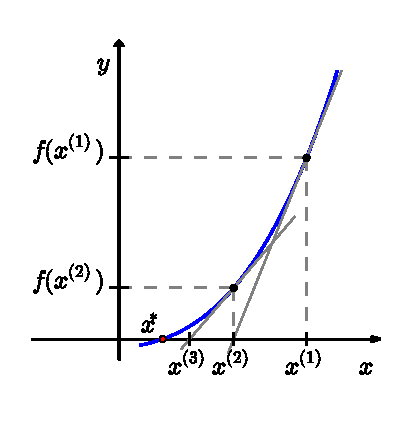
\includegraphics{metodo_de_Newton.eps}  
  \caption{Interpretação do método de Newton.}
  \label{fig:metodo_de_Newton}
\end{figure}

Ou seja, dada aproximação $x^{(n)}$, a próxima aproximação $x^{(n+1)}$ é o ponto de interseção entre o eixo das abscissas e a reta tangente ao gráfico da função no ponto $x = x^{(n)}$. Observe a Figura~\ref{fig:metodo_de_Newton}.

\subsection{Análise de convergência}\index{método de Newton-Raphson!convergência}\label{Analise_conv_Newton}

Seja $f(x)$ um função com derivadas primeira e segunda contínuas tal que $f(x^*)=0$ e $f'(x^*)\neq 0$. Seja também a função $g(x)$ definida como:
\begin{equation}
  g(x)=x-\dfrac{f(x)}{f'(x)}.
\end{equation}
Expandimos em série de Taylor em torno de $x = x^*$, obtemos:
\begin{equation}
  g(x)=g(x^*)+g'(x^*)(x-x^*) + \dfrac{g''(x^*)}{2}(x-x^*)^2 + O\left((x-x^*)^3\right).
\end{equation}
Observamos que:
\begin{eqnarray}
g(x^*) &=& x^*\\
g'(x^*) &=& 1 - \dfrac{f'(x^*)f'(x^*)-f(x^*)f''(x^*)}{\left(f'(x^*)\right)^2} = 0
\end{eqnarray}
Portanto:
\begin{equation}
g(x) = x^* + \dfrac{g''(x^*)}{2}(x-x^*)^2 + O\left((x-x^*)^3\right)\\
\end{equation}
Com isso, temos:
\begin{equation}
x^{(n+1)} = g(x^{(n)}) =  x^*+ \dfrac{g''(x^*)}{2}(x^{(n)}-x^*)^2 + O\left((x-x^*)^3\right),
\end{equation}
ou seja:
\begin{equation}
\left|x^{(n+1)}-x^*\right| \leq C\left|x^{(n)}-x^*\right|^2,
\end{equation}
com constante $C = \left|g''(x^*)/2\right|$. Isto mostra que o método de Newton tem \emph{taxa de convergência quadrática}. Mais precisamente, temos o seguinte teorema.

\begin{teo}[Método de Newton]
  Sejam $f\in C^2([a, b])$ com $x^*\in (a, b)$ tal que $f(x^*) = 0$ e:
  \begin{equation}
    m := \min_{x\in [a, b]}|f'(x)| > 0\quad\text{e}\quad M := \max_{x\in [a, b]} |f''(x)|.
  \end{equation}
Escolhendo $\rho > 0$ tal que:
\begin{equation}
  q := \dfrac{M}{2m}\rho < 1, 
\end{equation}
definimos a \emph{bacia de atração} do método de Newton pelo conjunto:
\begin{equation}
  K_\rho(x^*) := \left\{x\in\mathbb{R};~|x-x^*| \leq \rho\right\}\subset [a, b].
\end{equation}
Então, para qualquer $x^{(1)}\in K_\rho(x^*)$ a iteração do método de Newton:
\begin{equation}
  x^{(n+1)} = x^{(n)} - \dfrac{f(x^{(n)})}{f'(x^{(n)})},
\end{equation}
fornece uma sequência $x^{(n)}$ que converge para $x^*$, isto é, $x^{(n)}\to x^*$ quando $n\to \infty$. Além disso, temos a seguinte estimativa de erro \emph{a priori}:
\begin{equation}
  |x^{(n)} - x^*| \leq \dfrac{2m}{M}q^{(2^{n-1})},\quad n\geq 2,
\end{equation}
e a seguinte estimativa de erro \emph{a posteriori}:
\begin{equation}
  |x^{(n)} - x^*| \leq \dfrac{M}{2m}|x^{(n)} - x^{(n-1)}|^2,\quad n\geq 2.
\end{equation}
\end{teo}
\begin{proof}
  Para $n\in\mathbb{N}$, $n\geq 2$, temos:
  \begin{equation}\label{eq:forma}
    x^{n+1}-x^* = x^{(n)} - \dfrac{f(x^{(n)})}{f'(x^{(n)})} - x^* = -\dfrac{1}{f(x^{(n)})}\left[f(x^{(n)})+(x^*-x^{(n)})f'(x^{(n)}\right].
  \end{equation}
Agora, para estimar o lado direito desta equação, usamos o polinômio de Taylor de grau $1$ da função $f(x)$ em torno de $x = x^{(n)}$, isto é:
\begin{equation}
  f(x^*) = f(x^{(n)}) + (x^* - x^{(n)})f'(x^{(n)}) + \int_{x^{(n)}}^{x^*} f''(t)(x^* - t)\,dt.
\end{equation}
Pela mudança de variável $t = x^{(n)} + s(x^{(n)} - x^*)$, observamos que o resto deste polinômio de Taylor na forma integral é igual a:
\begin{equation}
  R(x^*,x^{(n)}) := (x^* - x^{(n)})^2\int_0^1 f''\left(x^{(n)} + s(x^* - x^{(n)})\right)(1-s)\,ds.
\end{equation}
Assim, da cota da segunda derivada de $f(x)$, temos:
\begin{equation}\label{eq:est-resto}
  |R(x^*,x^{(n)})| \leq M|x^*-x^{(n)}|^2\int_0^1 (1-s)\,ds = \dfrac{M}{2}|x^* - x^{(n)}|^2.
\end{equation}\label{eq:quadratica}
Se $x^{(n)}\in K_\rho(x^*)$, então de \eqref{eq:forma} e \eqref{eq:est-resto} temos:
\begin{equation}
  |x^{(n+1)} - x^*| \leq \dfrac{M}{2m}|x^{(n)} - x^*|^2 \leq \dfrac{M}{2m}\rho^2 < \rho.
\end{equation}
Isto mostra que se $x^{(n)}\in K_\rho(x^*)$, então $x^{(n+1)}\in K_\rho(x^*)$, isto é, $x^{(n)}\in K_\rho(x^*)$ para todo $n\in\mathbb{R}$.

Agora, obtemos a estimativa \emph{a priori} de \eqref{eq:quadratica}, pois:
\begin{equation}
  |x^{(n)} - x^*| \leq \dfrac{2m}{M}\left(\dfrac{M}{2m}|x^{(n-1)}-x^*|\right)^2 \leq \cdots \leq \dfrac{2m}{M}\left(\dfrac{M}{2m} |x^{(1)}-x^*|\right)^{2^{n-1}}.
\end{equation}
Logo:
\begin{equation}
  |x^{(n)} - x^*| \leq \dfrac{2m}{M}q^{2^{n-1}},
\end{equation}
donde também vemos que $x^{(n)}\to x^*$ quando $n\to\infty$, pois $q < 1$.

Por fim, para provarmos a estimativa \emph{a posteriori} tomamos a seguinte expansão em polinômio de Taylor:
\begin{equation}
  f(x^{(n)}) = f(x^{(n-1)}) + (x^{(n)} - x^{(n-1)})f'(x^{(n-1)}) + R(x^{(n)},x^{(n-1)}).
\end{equation}
Aqui, temos:
\begin{equation}
  f(x^{(n-1)}) + (x^{(n)} - x^{(n-1)})f'(x^{(n-1)}) = 0
\end{equation}
e, então, conforme acima:
\begin{equation}
  |f(x^{(n)})| = |R(x^{(n)}),x^{(n-1)}| \leq \dfrac{M}{2}|x^{(n)} - x^{(n-1)}|^2.
\end{equation}
Com isso e do teorema do valor médio, concluímos:
\begin{equation}
  |x^{(n)} - x^*| \leq \dfrac{1}{m}|f(x^{(n)}) - f(x^*)| \leq \dfrac{M}{2m}|x^{(n)} - x^{(n-1)}|^2.
\end{equation}
\end{proof}

\begin{ex}
  Estime o raio $\rho$ da bacia de atração $K_\rho(x^*)$ para a função $f(x) = \cos(x) - x$ restrita ao intervalo $[0, \pi/2]$.
\end{ex}
\begin{sol}
  O raio da bacia de atração é tal que:
  \begin{equation}
    \rho < \dfrac{2m}{M}
  \end{equation}
onde $m := \min |f'(x)|$ e $M := \max |f''(x)|$ com o mínimo e o máximo tomados em um intervalo $[a, b]$ que contenha o zero da função $f(x)$. Aqui, por exemplo, podemos tomar $[a, b] = [0, \pi/2]$. Como, neste caso, $f'(x) = -\sin(x) - 1$, temos que $m = 1$. Também, como $f''(x) = -\cos x$, temos $M = 1$. Assim, concluímos que $\rho < 2$ (lembrando que $K_\rho(x^*)\subset [0, \pi/2]$). Ou seja, neste caso as iterações de Newton convergem para o zero de $f(x)$ para qualquer escolha da aproximação inicial $x^{(1)}\in [0, \pi/2]$.
\end{sol}

\section{Método Quasi-Newton}\index{método Quasi-Newton}
Para descrever este método, suponha que uma aproximação inicial $x^{(0)}$ seja dada para a solução \textit{p} de $F\left(x\right)=0$. Calculamos a aproximação seguinte $x^{{1}}$ do mesmo modo que no método de Newton, ou, se for inconveniente determinar $J\left(x^{(0)}\right)$ exatamente, utilizamos as equações de diferença dadas pela Equação abaixo:
$$\dfrac{\partial f_j}{\partial x_k}\left(x^{(i)}\right)\approx\dfrac{f_j\left(x^{(i)}+e_kh
\right)-f_j\left(x^{(i)}\right)}{h}$$

Para aproximar as derivadas parciais. Para calcular $x^{2}$,'contudo, saímos do método de Newton e examinamos o método as Secantes para uma única equação não-linear. O método das Secantes usa a aproximação:
$$f'(x_1)\approx\dfrac{f\left(x_1\right)-f\left(x_0\right)}{x_1-x_0}$$

Como uma substituição para $f'\left(x_1\right)$ no método de Newton. Para sistemas não-lineares, $x^{1}-x^{(0)}$ é um vetor e o quociente correspondente não é definido. Todavia, o método prossegue analogamente quanto a substituirmos na matriz $J\left(x^{(1)}\right)$ no método de Newton para sistemas por uma matriz $A_1$ com a propriedade que:
$$A_1\left(x^{\left(1\right)}-x^{\left(0\right)}\right)=F\left(x^{\left(1\right)}
\right)-F\left(x^{\left(0\right)}\right)$$

Qualquer vetor diferente de zero em ${\mathbb{R}}^n$ pode ser escrito como a soma de um múltiplo de $x^{1}-x^{(0)}$ com um múltiplo de um vetor no complemento ortogonal de $x^{1}-x^{(0)}$. Assim, para definirmos de $x^{1}-x^{\left(0\right)}$, já que nenhuma informação está disponível a respeito da variação em $F$ em uma direção ortogonal a $x^{1}-x^{(0)}$, exigimos que:
\begin{center}
$A_1z=J\left(x^{(0)}\right)z,$ sempre que ${\left(x^{(1)}-x^{\left(0\right)}\right)}^t$ $z=0.$ 
\end{center}

Assim, qualquer vetor ortogonal a $x^{1}-x^{(0)}$ não é afetado pela atualização de $J\left(x^{(0)}\right)$, que foi usada para calcular $x^{1}$, para $A_1$, que foi usada na determinação de $x^{2}$.

As condições acima definem $A_1$ de modo único, como:
$$A_1=J\left(x^{(0)}\right)+\dfrac{\left[F\left(x^{\left(1\right)}\right)-F\left(x^{\left(0\right)}\right)-J\left(x^{\left(0\right)}\right)\left(x^{\left(1\right)}-x^{\left(0\right)}\right)\right]{\left(x^{(1)}-x^{\left(0\right)}\right)}^t}{{\left\|x^{(1)}-x^{\left(0\right)}\right\|}^2_2}$$
é esta matriz que é utilizada no lugar de $J\left(x^{\left(1\right)}\right)$ para se determinar $x^{\left(2\right)}$ como:
$$x^{\left(2\right)}=x^{\left(1\right)}-A^{-1}_1F\left(x^{\left(1\right)}\right).$$

Uma vez que $x^{\left(2\right)}$ tenha sido determinado, o método é repetido para determinar $x^{\left(3\right)},$ usando $A_1$ no lugar de $A_0=J\left(x^{\left(0\right)}\right)$, e como $x^{\left(2\right)}$ e $x^{\left(1\right)}$ no lugar de $x^{\left(1\right)}$ e $x^{\left(0\right)}$. Em geral, uma vez que $x^{\left(i\right)}$ tenha sido determinado, $x^{\left(i+1\right)}$ é calculado por:
$$A_i=A_{i-1}+\dfrac{y_i-A_{i-1}s_i}{{\left\|s_i\right\|}^2_2}{s_i}^t$$ $$x^{\left(i+1\right)}=x^{\left(i\right)}-A^{-1}_1F\left(x^{\left(i\right)}\right),$$

Em que a notação $y_i=F\left(x^{\left(i\right)}\right)-F\left(x^{\left(i-1\right)}\right)$ e $s_i=x^{\left(i\right)}-x^{\left(i-1\right)}$ é introduzida para simplificar as equações.

Se o método for realizado como delineado nas equações aimca, a quantidade de cálculos de funções escalares ficará reduzida de $n^2+n$ para $n$(aquelas necessárias para calcular $F\left(x^{\left(i\right)}\right)$), mas cálculos de $O\left(n^3\right)$ ainda são necessários para resolver o sistema linear $n\ x\ n$ associado.
$$A_is_{i+1}=-F\left(x^{(i)}\right)$$

O emprego do método nesta forma não seria justificado por causa da redução para convergência super linear a partir da convergência quadrática do método de Newton.

\newpage
\chapter{Resultados}\index{Resultados}
Sobre os testes com o sistema tridiagonal de Broyden, temos os resultados para os seguintes tópicos:
%%-------------------------------------------------------------------------------------
\section{O grau e o padrão de esparsidade da matriz jacobiana}\index{O grau e o padrão de esparsidade da matriz jacobiana}

O grau e o padrão de esparsidade da matriz jacobiana para $p = 1000$. Com base nestes resultados identificando se a matriz jacobiana é densa ou esparsa.

Primeiramente, iremos discutir um pouco sobre esparsidade, mostrando como se calcula seu grau e seu padrão: 
 
\subsection{GRAU DE ESPARSIDADE} 
 
Para calcular o grau de esparsidade, levemos em consideração que este grau é uma métrica que informa a percentagem dos elementos nulos da matriz. Daí, seja $G_S$ grau de esparsidade. Pode-se escrever:

$$G_S = \dfrac{p^2-N}{p^2}$$
  
Onde $N$ é o número de elementos não-nulos e $p$ é a ordem da matriz quadrada cujo grau de esparsidade será extraído. 

Para o jacobiano do sistema de Broyden, tem-se 2 elementos não nulos na primeira e na última linha. Nas $p-2$ linhas intermediárias, tem-se 3 elementos não nulos. Daí: 
$$N=3\cdot(p-2)+4=3p-2$$

Portanto,
$$G_S=\dfrac{p^2-(3p-2)}{p^2}=\dfrac{p^2-3p+2}{p^2}$$
  
Para o caso particular em que $p=1000$ tem-se: 
$$G_S=\dfrac{1000^2-(3\cdot1000+2)}{1000^2}\cdot100\%=99.7002\%$$

Desta forma, como a maior parte dos elementos do jacobiano é nula, esta matriz é esparsa. 

\newpage
%%-------------------------------------------------------------------------------------
\section{Solução do sistema de Broyden - primeiro caso}\index{Solução do sistema de Broyden - primeiro caso}
A solução do sistema de Broyden para p = 5, 10 e 20 usando o Método de Newton-Raphson. Apresente o vetor solução, os valores finais de $||F(x)||_\infty$ e também o número de iterações realizadas.
\subsection{Para p = 5:}

Iterações: 3

$||F(x)||_\infty=6.6411\times10^{-9}$

Vetor Solução:
\begin{eqnarray}
      X =
    \begin{bmatrix}
      -0.9684\\
      -1.1870\\
      -0.9590\\
      -0.5942
    \end{bmatrix}.
    \end{eqnarray}
\subsection{Para p = 10:}

Iterações: 3

$||F(x)||_\infty=6.3098\times10^{-7}$

Vetor Solução:
\begin{eqnarray}
      X =
    \begin{bmatrix}
      -1.0301\\
      -1.3104\\
      -1.3799\\
      -1.3907\\
      -1.3796\\
      -1.3499\\
      -1.2907\\
      -1.1775\\
      -0.9675\\
      -0.5965\\
    \end{bmatrix}.
    \end{eqnarray}
\newpage

\subsection{Para p = 20:}

Iterações: 4

$||F(x)||_\infty=1.8145\times10^{-12}$

Vetor Solução:
\begin{eqnarray}
      X =
    \begin{bmatrix}
      -1.03024\\
      -1.3150\\
      -1.3887\\
      -1.4076\\
      -1.4125\\
      -1.4137\\
      -1.4139\\
      -1.4139\\
      -1.4136\\
      -1.4130\\
      -1.4119\\
      -1.4098\\
      -1.4055\\
      -1.3973\\
      -1.3813\\
      -1.3504\\
      -1.2908\\
      -1.1775\\
      -0.9675\\
      -0.5965\\
    \end{bmatrix}.
    \end{eqnarray}

\newpage
%%-------------------------------------------------------------------------------------
\section{Solução do sistema de Broyden - segundo caso}\index{Solução do sistema de Broyden - segundo caso}

Para $p = 5$, foram necessário 8 iterações, sendo $|| F_x ||_\infty = 3,2873e-007$, e encontrado a seguinte solução:
\begin{table}[h]
    \vspace*{0,2cm}
    \centering
    \caption{Valores de X para $p = 5$.}
    \begin{tabular}{|c|r|}\hline
        \multicolun {X} & {Resultado} \\\hline
        {$X(2)$} & $-1,1870$\\\hline
        {$X(3)$} & $-1,1485$\\\hline
        {$X(4)$} & $-0,9590$\\\hline
        {$X(5)$} & $-0,5942$\\\hline
    \end{tabular}
\end{table}

Para $p = 10$, foram necessário 10 iterações, sendo $|| F_x ||_\infty = 6,2736e-007$ , e encontrado a seguinte solução:

\begin{table}[h]
    \vspace*{0,2cm}
    \centering
    \caption{Valores de X para $p = 10$.}
    \begin{tabular}{|c|r|}\hline
        \multicolun {X} & {Resultado} \\\hline
        {$X(1)$} & $-1,0301$\\\hline
        {$X(2)$} & $-1,3104$\\\hline
        {$X(3)$} & $-1,3799$\\\hline
        {$X(4)$} & $-1,3907$\\\hline
        {$X(5)$} & $-1,3796$\\\hline
        {$X(6)$} & $-1.3499$\\\hline
        {$X(7)$} & $-1.2907$\\\hline
        {$X(8)$} & $-1.1775$\\\hline
        {$X(9)$} & $-0.9675$\\\hline
        {$X(10)$} & $-0,5965$\\\hline
    \end{tabular}
\end{table}

\newpage
Para $p = 20$, foram necessário 10 iterações, sendo $|| F_x ||_\infty = 7.9266e-007$ , e encontrado a seguinte solução:

\begin{table}[h]
    \vspace*{0,2cm}
    \centering
    \caption{Valores de X para $p = 20$.}
    \begin{tabular}{|c|r|}\hline
    \multicolun { X } & { Resultado } \\\hline
        {$X(1)$} & $-1,0324$ \\\hline
        {$X(2)$} & $-1,3150$ \\\hline
        {$X(3)$} &  $-1,3887$ \\\hline
        {$X(4)$} &  $-1,4076$ \\\hline
        {$X(5)$} &  $-1,4125$ \\\hline
        {$X(6)$} &  $-1,4137$ \\\hline
        {$X(7)$} &  $-1,4139$ \\\hline
        {$X(8)$} &  $-1,4138$ \\\hline
        {$X(9)$} &  $-1,4136$ \\\hline
        {$X(10)$} & $-1,4130$ \\\hline
        {$X(11)$} & $-1,4119$  \\\hline
        {$X(12)$} & $-1,4098$  \\\hline
        {$X(13)$} & $-1,4055$  \\\hline
        {$X(14)$} & $-1,3973$  \\\hline
        {$X(15)$} & $-1,3813$  \\\hline
        {$X(16)$} & $-1,3504$  \\\hline
        {$X(17)$} & $-1,2908$  \\\hline
        {$X(18)$} & $-1,1775$  \\\hline
        {$X(19)$} & $-0,9675$  \\\hline
        {$X(20)$} &  $-0,5965$ \\\hline
    \end{tabular}
\end{table}

\newpage
%%-------------------------------------------------------------------------------------
\section{Comparação dos resultados com o \MATLAB}\index{Comparação dos resultados com o \MATLAB}

Compare os resultados obtidos nas seções 2 e 3 com aqueles obtidos pela função nativa do \MATLAB para a solução de sistemas não-lineares. Apresente uma descrição resumida do método usado pela função nativa do \MATLAB para solução de sistemas não-lineares.

Nas três tabelas a baixos estão as comparações das soluções do sistema de Broyden, com quatro casas de precisão, para p = 5, 10 e 20. Foram utilizados os métodos de Newton-Raphson, Newton Modificado (Quase-Newton) e a função nativa do \MATLAB fsolve \cite{matworks}.

A função fsolve é uma função nativa do \MATLAB robusta que implementa três algorítimos diferentes: trust region dogleg, trust region e Levenberg-Marquardt \cite{matsumoto}. Ela possui variações de entradas, porém a utilizada foi X = fsolve (FUN, X0).

Os resultados para quatro casas de precisão e com tolerância 1*10$\mathrm{\wedge}$-6 foram os mesmos para as três tabelas. Contudo as  diferenças mais acentuadas foram no número de interações, sendo a QuasiNewton nas três tabelas apresentou um numero de interações maior que o dobro das outras duas.  Para os tamanhos  utilizados o método de Newton-Raphson e a função   fsolve obtiveram o mesmo número de interações. Nos algoritmos implementados também foi utilizado a cputime para medir o tempo. Embora o tempo não tenha se mantido constante para ser posto na tabela foi possível observar que a conseguia os resultados de forma mais rápida que o método Newton-Raphson.  Em relação as normas que mostram o quanto foi preciso os cálculos. é possível observar que utilizando Newton Modificado a norma nas três tabelas foi maior que os outros dois métodos. E entre a função nativa do \MATLAB e Newton-Raphson obtiveram bons resultados, variando em qual se saiu melhor nas três tabelas.

\begin{table}[h]
    \vspace*{0,2cm}
    \centering
    \caption{Primeira comparação com o \MATLAB.}
    \begin{tabular}{|c|c|c|c|} \hline 
    $p=5$ & Newton\_Raphson & Quasi\_Newton & \textit{fsolve} \\ \hline 
    Solução $x$ & $\left[ \begin{array}{c}
    \ -0.9684 \\ 
    -1.1870 \\ 
    -1.1485 \\ 
    -0.9590 \\ 
    -0.5942 \end{array}
    \right]$ & $\left[ \begin{array}{c}
    \ -0.9684 \\ 
    -1.1870 \\ 
    -1.1485 \\ 
    -0.9590 \\ 
    -0.5942 \end{array}
    \right]$ & $\left[ \begin{array}{c}
    \ -0.9684 \\ 
    -1.1870 \\ 
    -1.1485 \\ 
    -0.9590 \\ 
    -0.5942 \end{array}
    \right]$ \\ \hline 
    \newline Nº de iterações\newline  & 3 & 9 & 3 \\ \hline 
    Solução inicial & \newline $\mathrm{-}\mathrm{ones(5,1}$)\newline  & \newline $\mathrm{-}\mathrm{ones(5,1)}$ & \newline $\mathrm{-}\mathrm{ones(5,1)}$ \\ \hline 
    \newline Tolerância\newline  & ${1.10}^{-6}$ & ${1.10}^{-6}$ & ${1.10}^{-6}$ \\ \hline 
    ${\left|\left|F\left(x\right)\right|\right|}_{\infty }$ & $6,6411\cdot {10}^{-9}$ & $3,3131.{10}^{-7}$ & $\mathrm{6.6392}\cdot {10}^{-9}$ \\ \hline 
    \end{tabular}
\end{table}

\newpage

\begin{table}[h]
    \vspace*{0,2cm}
    \centering
    \caption{Segunda comparação com o \MATLAB.}
    \begin{tabular}{|c|c|c|c|} \hline 
    $p=10$ & Newton\_Raphson & Quasi\_Newton & \textit{fsolve} \\ \hline 
    \newline Solução $x$\newline  & \newline $\left[ \begin{array}{c}
    \ -1.0301 \\ 
    -1.3104 \\ 
    -1.3799 \\ 
    -1.3907 \\ 
    -1.3796 \\ 
    -1.3499 \\ 
    -1.2907 \\ 
    -1.1775 \\ 
    -0.9675 \\ 
    -0.5965 \end{array}
    \right]$\newline  & $\left[ \begin{array}{c}
    \ -1.0301 \\ 
    -1.3104 \\ 
    -1.3799 \\ 
    -1.3907 \\ 
    -1.3796 \\ 
    -1.3499 \\ 
    -1.2907 \\ 
    -1.1775 \\ 
    -0.9675 \\ 
    -0.5965 \end{array}
    \right]$ & $\left[ \begin{array}{c}
    \ -1.0301 \\ 
    -1.3104 \\ 
    -1.3799 \\ 
    -1.3907 \\ 
    -1.3796 \\ 
    -1.3499 \\ 
    -1.2907 \\ 
    -1.1775 \\ 
    -0.9675 \\ 
    -0.5965 \end{array}
    \right]$ \\ \hline 
    \newline Nº de iterações\newline  & 3 & 10 & 3 \\ \hline 
    Solução inicial & \newline $\mathrm{-}\mathrm{ones(10,1}$)\newline  & \newline $\mathrm{-}\mathrm{ones(10,1)}$ & \newline $\mathrm{-}\mathrm{ones(10,1)}$ \\ \hline 
    \newline Tolerância\newline  & ${1.10}^{-6}$ & ${1.10}^{-6}$ & ${1.10}^{-6}$ \\ \hline 
    ${\left|\left|F\left(x\right)\right|\right|}_{\infty }$ & $6,3098\cdot {10}^{-7}$ & $\mathrm{1.9219}{.10}^{-7}$ & $\mathrm{3.0453}\cdot {10}^{-8}$ \\ \hline 
    \end{tabular}
\end{table}

\newpage

\begin{table}[h]
    \vspace*{0,2cm}
    \centering
    \caption{Terceira comparaçao com o \MATLAB.}
    \begin{tabular}{|c|c|c|c|} \hline 
    $p=20$ & Newton\_Raphson & Quasi\_Newton & \textit{fsolve} \\ \hline 
    \newline Solução $x$\newline  & \newline $\left[ \begin{array}{c}
    -1.0324 \\ 
    -1.3150 \\ 
    -1.3887 \\ 
    -1.4076 \\ 
    -1.4125 \\ 
    -1.4137 \\ 
    -1.4139 \\ 
    -1.4139 \\ 
    -1.4136 \\ 
    -1.4130 \\ 
    -1.4119 \\ 
    -1.4098 \\ 
    -1.4055 \\ 
    -1.3973 \\ 
    -1.3813 \\ 
    -1.3504 \\ 
    -1.2908 \\ 
    -1.1775 \\ 
    -0.9675 \\ 
    -0.5965 \end{array}
    \right]$\newline  & $\left[ \begin{array}{c}
    -1.0324 \\ 
    -1.3150 \\ 
    -1.3887 \\ 
    -1.4076 \\ 
    -1.4125 \\ 
    -1.4137 \\ 
    -1.4139 \\ 
    -1.4139 \\ 
    -1.4136 \\ 
    -1.4130 \\ 
    -1.4119 \\ 
    -1.4098 \\ 
    -1.4055 \\ 
    -1.3973 \\ 
    -1.3813 \\ 
    -1.3504 \\ 
    -1.2908 \\ 
    -1.1775 \\ 
    -0.9675 \\ 
    -0.5965 \end{array}
    \right]$ & $\left[ \begin{array}{c}
    -1.0324 \\ 
    -1.3150 \\ 
    -1.3887 \\ 
    -1.4076 \\ 
    -1.4125 \\ 
    -1.4137 \\ 
    -1.4139 \\ 
    -1.4139 \\ 
    -1.4136 \\ 
    -1.4130 \\ 
    -1.4119 \\ 
    -1.4098 \\ 
    -1.4055 \\ 
    -1.3973 \\ 
    -1.3813 \\ 
    -1.3504 \\ 
    -1.2908 \\ 
    -1.1775 \\ 
    -0.9675 \\ 
    -0.5965 \end{array}
    \right]$ \\ \hline 
    \newline Nº de iterações\newline  & 4 & 10 & 4 \\ \hline 
    Solução inicial & \newline $\mathrm{-}\mathrm{ones(20,1)}$\newline  & \newline $\mathrm{-}\mathrm{ones(20,1)}$ & \newline $\mathrm{-}\mathrm{ones(20,1)}$ \\ \hline 
    \newline Tolerância\newline  & ${1.10}^{-6}$ & ${1.10}^{-6}$ & ${1.10}^{-6}$ \\ \hline 
    ${\left|\left|F\left(x\right)\right|\right|}_{\infty }$ & $1.8145\cdot {10}^{-12}$ & 7.9266${10}^{-7}$ & $\mathrm{8.5744}\cdot {10}^{-10}$ \\ \hline 
    \end{tabular}
\end{table}

\newpage
%%-------------------------------------------------------------------------------------
\section{Avaliação do custo computacional}\index{Avaliação do custo computacional}
Avaliação do custo computacional (tempo de processamento) para o obter a solução do sistema de broyden com $p = 1000$ para os seguintes métodos: método de Newton-Raphson, método de Newton modificado e o método usado pela função nativa do \MATLAB.

Na tabela, são computados os tempos de processamento de cada um dos métodos e da função \textit{fsolve}\cite{matworksfsolve}, onde notamos um contrabalanceamento por parte do método de Quasi-Newton, que obteve um tempo de processamento muito menor que do método de Newton-Raphson, devido a maior complexidade deste. Apesar da função \textit{fsolve} também ser implementada de forma complexa, seu tempo de processamento foi bem próximo ao do método de Quasi-Newton, pois fsolve resolveu o sistema através do método \textit{trust-region dogleg.}

\begin{table}[h]
    \vspace*{0,2cm}
    \centering
    \begin{tabular}{|c|c|} \hline 
    $P = 1000$ & Tempo de Processamento (segundos) \\ \hline 
    Newton-Raphson & $130.4324$ \\ \hline 
    Quase-Newton & $42.2919$ \\ \hline 
    \textit{fsolve} & $4.2276$ \\ \hline 
    \end{tabular}
\end{table}

Para entender como a função nativa é tão mais rápida quanto a Newton-Raphson e Quase-Newton, basta entender que a solução que o \MATLAB impõe. Isto é, mescla-se o método de mínimos quadrados para adaptar e reduzir a função por uma menor, além de usar série de Taylor também para manipular a função e ocasionar novas aproximações e o método de gradiente.

Toda esta adaptação é para que o \MATLAB convirja os cálculos para algo matricial. A adaptação final da aproximação para uma dada função $F_i\left(x\right)=0$ com todas as técnicas de minimização, resultando em ${\mathrm{min} \{\frac{1}{2}s^THs+s^Tg\ such\ that\ \left|\left|Ds\right|\right|\le \Delta \ }$ onde H é a matriz Hessiana, g é o gradiente da função e D a matriz diagonal, $\Delta $ é um valor numérico escalar. Ademais, é utilizado os autovalores e autovetores da função $F_i(x)$ definida na forma matricial. Concluindo, então, usando o próprio método de Newton.

O \MATLAB, portanto, através do $fsolve$ consegue misturar métodos de funções não lineares (método de Newton) com os métodos lineares (gradientes e uso de autovalores e autovetores, diagonalização de matriz, etc.). Tanto o método de Newton-Raphson quanto de Broyden apresentam uma complexidade superior à O(n$\mathrm{\wedge}$2). Isso porque além dos laços para varrimento de linhas e colunas, apresentam lógicas de condições dentro destes, acarretando numa lentidão natural por parte do \MATLAB. Entretanto, evita-se o tratamento do método com matrizes inversas cujo custo poderia ser ainda maior. O mesmo pensamento de vetorização e tratamento matricial do código diminuí o custo computacional.
\newpage
%=================================================================================================================================================
\chapter{Conclusões}\index{Conclusões}

A aprendizagem e o domínio dos métodos de Newton-Raphson e Quasi-Newton são de grande importância para determinar com eficiência a resolução de problemas que envolvam a solução de sistemas não lineares. O método de Newton-Raphson apresenta convergência do processo iterativo mais rápida. Isso o torna mais vantajoso em relação aos métodos anteriormente estudados. O método de Newton modificado tem a vantagem de calcular uma única vez a matriz Jacobiana. No caso de resolver por fatoração LU, os fatores L e U serão calculados uma única vez. Esse método se mostrou ineficaz para sistemas com $p\geq10$. Por isso foi implementado o método de Quasi-Newton proposto por Broyden. É importante destacar que a ferramenta \MATLAB foi de grande auxílio na resolução dos problemas propostos porém estes métodos podem ser implementado de forma semelhante em outras linguagens como \textit{C++, Julia, Phyton}, entre outras. Como o programa foi dividido em funções, a resolução da matriz jacobiana e o cálculo das normas foram feitas de forma satisfatória, bem como o sistema de equações não-lineares testadas no sistema tridiagonal de Broyden. Na grande maioria das resoluções de sistemas não-lineares o método de Quasi-Newton pode assim apresentar um melhor desempenho.

%=================================================================================================================================================
%=================================================================================================================================================

% ----------------------------------------------------------
% Finaliza a parte no bookmark do PDF
% para que se inicie o bookmark na raiz
% e adiciona espaço de parte no Sumário
% ----------------------------------------------------------
\phantompart

% ----------------------------------------------------------
% ELEMENTOS PÓS-TEXTUAIS
% ----------------------------------------------------------
\postextual
% ----------------------------------------------------------

% ----------------------------------------------------------
% Referências bibliográficas
% ----------------------------------------------------------
\bibliography{references}

%\appendix
%\chapter{Apêndice}
%Este é o conteúdo do APÊNDICE A.
\begin{apendicesenv}
\partapendices
\chapter{Códigos Fonte}
\lstlistoflistings
\newpage
A seguir temos os códigos fonte feito neste trabalho:

\lstinputlisting[style=Matlab-editor, caption={BroydenFunção }]{broyden.m}
\lstinputlisting[style=Matlab-editor, caption={Função Norm-inf}]{norm_inf.m}\newpage
\lstinputlisting[style=Matlab-editor, caption={Função Jacobian}]{jacobian.m}\newpage
\lstinputlisting[style=Matlab-editor, caption={Função Jacobian-Broyden}]{jacobian_broyden.m}\newpage
\lstinputlisting[style=Matlab-editor, caption={Função LUGauss-Fac}]{lugauss_fac.m}
\lstinputlisting[style=Matlab-editor, caption={Função Mult}]{mult.m}\newpage
\lstinputlisting[style=Matlab-editor, caption={Função LUGauss-Sol}]{lugauss_sol.m}\newpage
\lstinputlisting[style=Matlab-editor, caption={Função main}]{main.m}\newpage
\lstinputlisting[style=Matlab-editor, caption={Função mainQuasiNewton}]{mainQuasi.m}\newpage
\lstinputlisting[style=Matlab-editor, caption={Newton-Raphson}]{newton_raphson.m}\newpage
\lstinputlisting[style=Matlab-editor, caption={Função Quasi2}]{quasi2.m}
\lstinputlisting[style=Matlab-editor, caption={Função Sub}]{sub.m}\newpage
\lstinputlisting[style=Matlab-editor, caption={Função Sum-Mat}]{sum_mat.m}
\lstinputlisting[style=Matlab-editor, caption={Função Transp}]{transp.m}
\end{apendicesenv}


\end{document}
%%% FIM %%%%%%%%%%%%%%%%%%%%%%%%%%%%%%%%%%%%%%%%%%%%%%%%%%%%%%%%%%%%%%%%%%%%%%%%%%%%%%%%%%%%%%%%%%%%%%%%